\item Wir betrachten die DGL $yy'+x-2y'=3$ und wollen das Richungsfeld skizzieren, für x- und y-Werte im Intervall $[0,5]$.
\begin{enumerate}
\item Formen Sie die DGL in explizite Form um, d.h. stellen Sie um nach $y'$.
\item Für das Richtungsfeld ist der Anstieg an verschiedenen Punkten zu berechnen. Um die Arbeit zu verringern, betrachten wir, an welchen Stellen der Anstieg $y'$ konstant ist. Dort zeigt das Richtungsfeld in die gleiche Richtung. Stellen Sie die Gleichung $y'=c$ (c: beliebige Konstante) nach $y(x)$ um.
\item Zeichnen Sie die so erhalten Funktionen $y(x)$ für $c\in\lbrace-5;-2;-0.5,-0,1;1,5\rbrace$. Zeichnen Sie zudem das Richtungfeld entlang diesen Funktionen. Anmerkung: Kurven, auf denen $y'=const$ gilt, nennt man Isoklinen (von lat. in\textbf{clin}are, engl. in\textbf{clin}ation, "Neigung").
\item Ermitteln Sie graphisch die Lösung der DGL für $(i)$ das Anfangswertproblem $y(4)=2$ und $(ii)$ für das Anfangswertproblem $y(1) = 1$. Um was für ein geometrisches Objekt handelt es sich bei den Lösungen?
\item Veranschaulichen Sie sich die Lösung mittels dem Online-Tool \href{https://www.geogebra.org/m/W7dAdgqc}{Geogebra}. Für den Anfangswert $y(2)=3$ zeigt dieses Tool (s. Abbildung \ref{ex-ode-slope-field-1-img-a}) links und rechts unerwartete Sprünge. Können Sie sich dieses Verhalten erklären? (Hinweis: Die Gleitkommazahlen stellen eine abzählbare, endliche Menge dar.)
\end{enumerate}


\begin{figure}[ht]
	\centering
	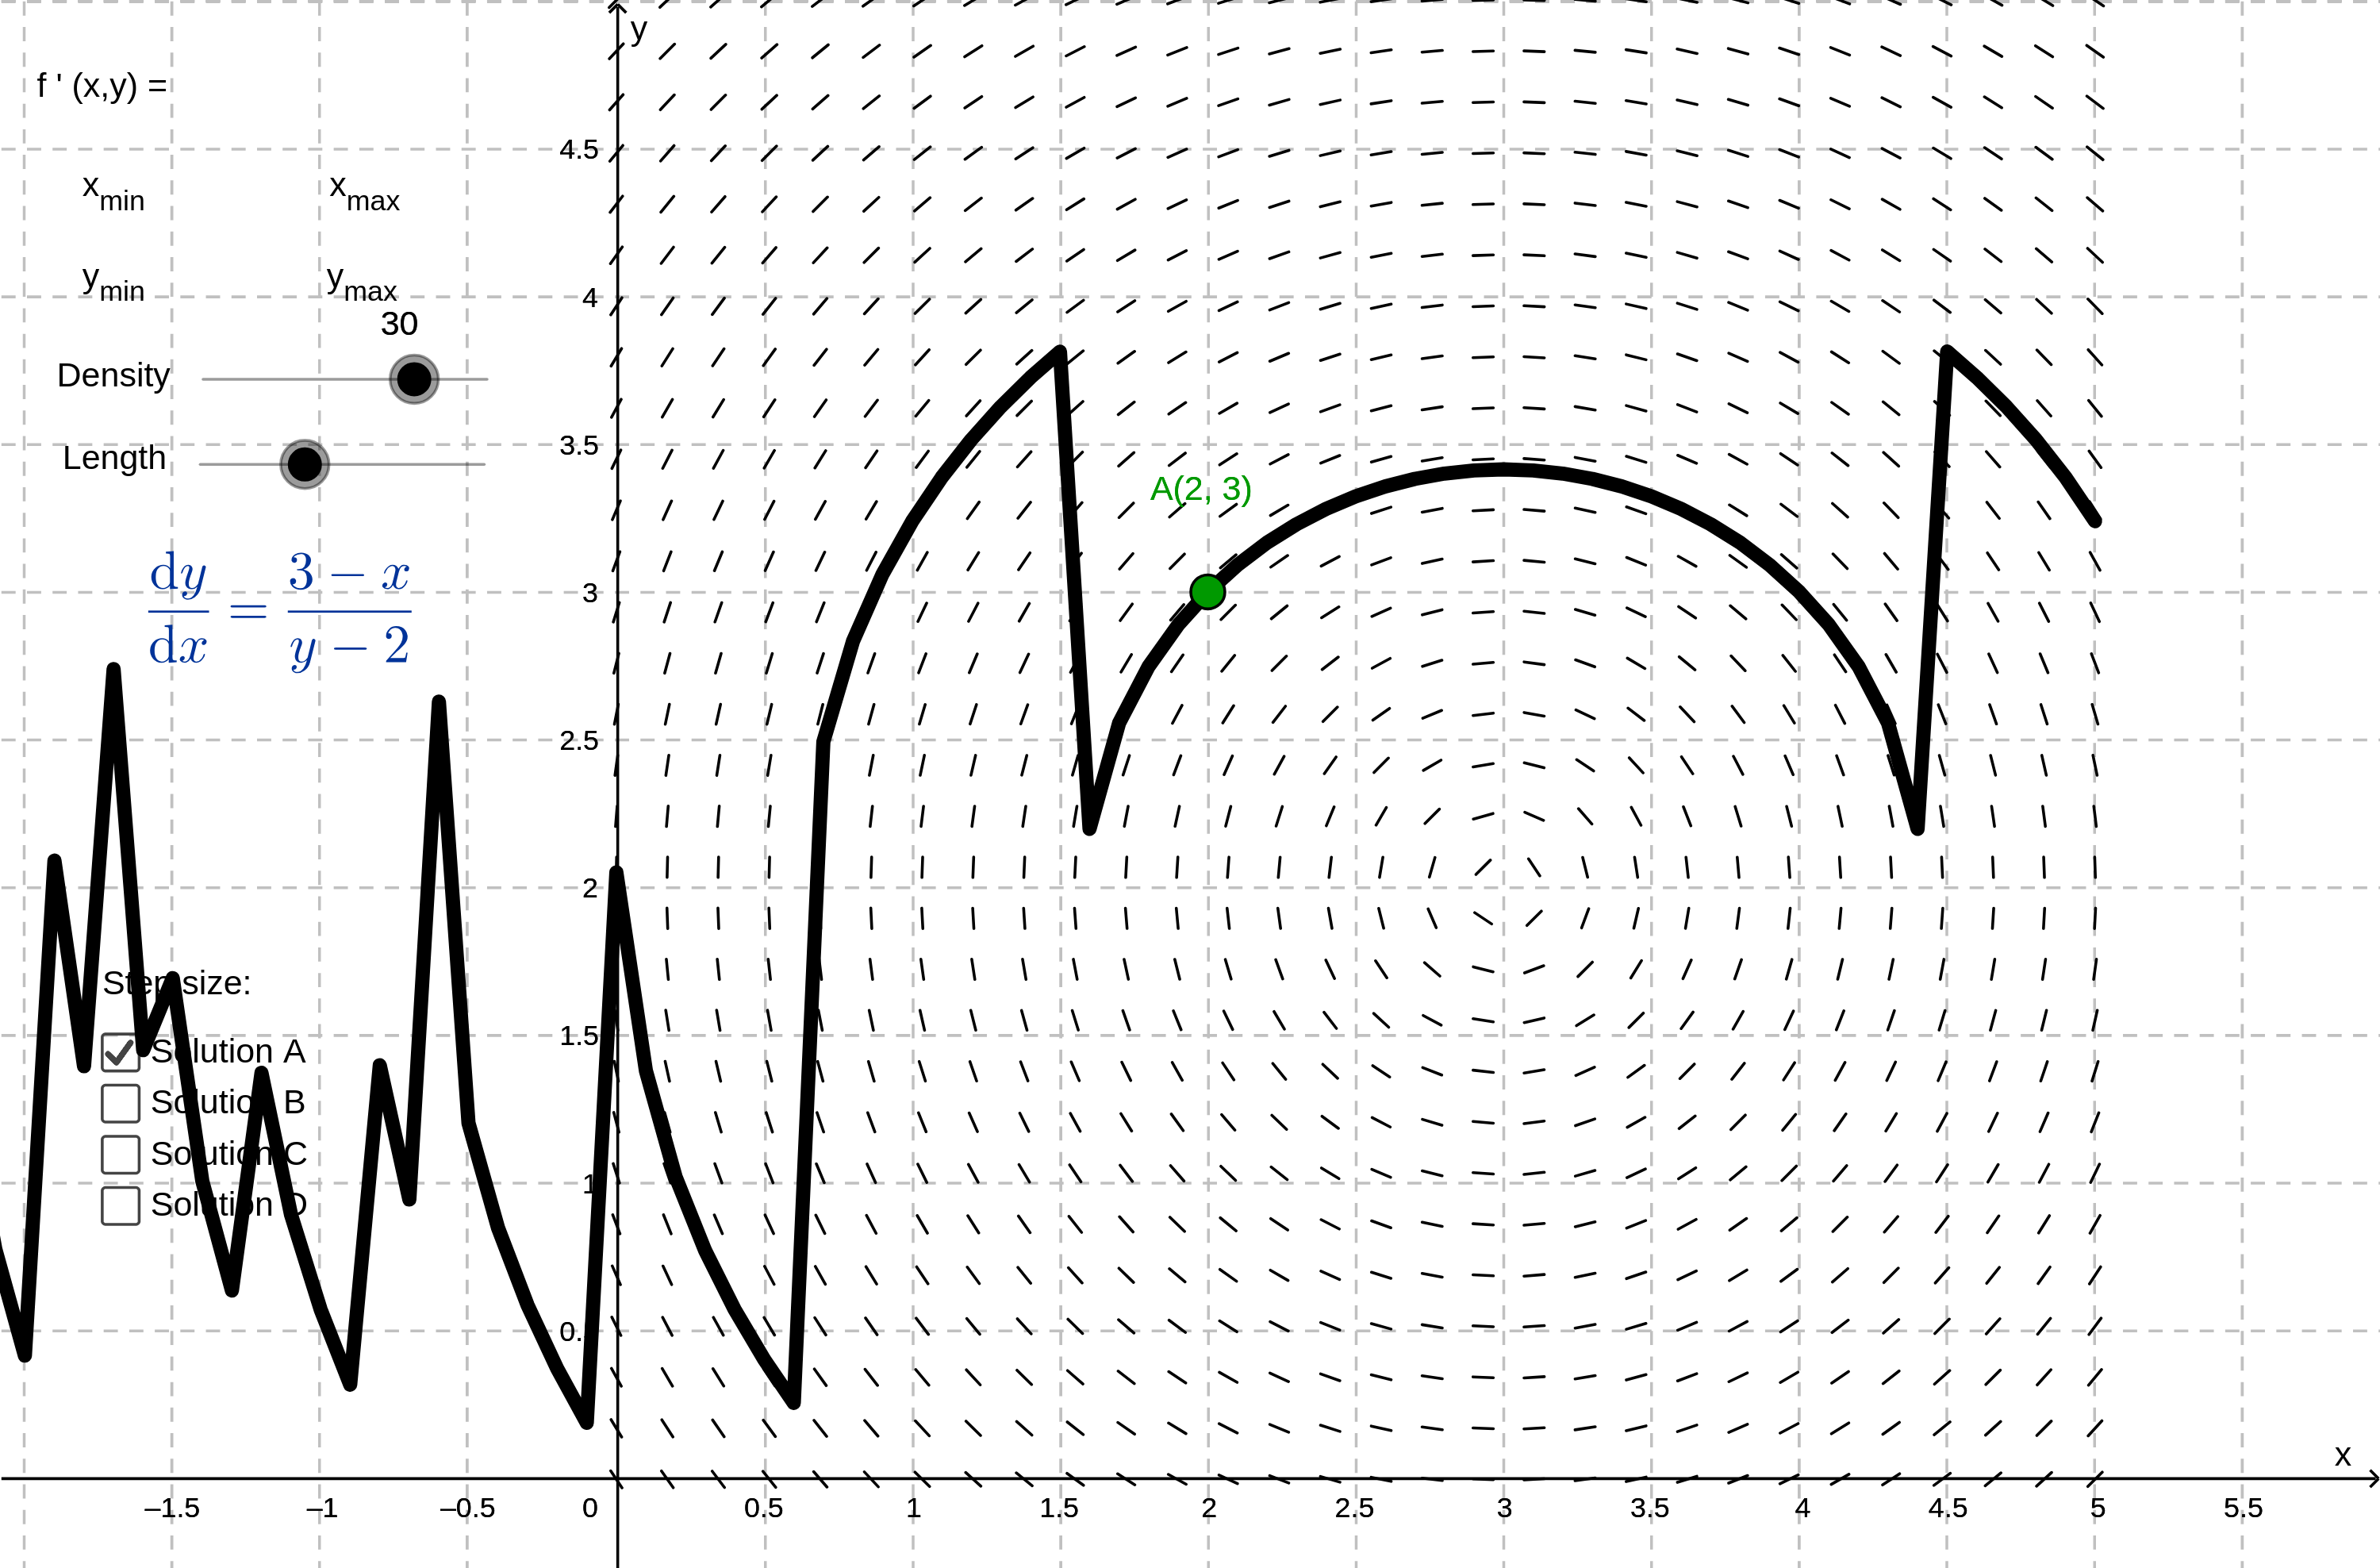
\includegraphics[width=0.45\textwidth]{../tex-snippets/ex-ode-slope-field-1-img-a.png}
	\caption{Numerische Lösung der DGL aus Aufgabe 1.5 mittels Geogebra für den Anfangswert $y(2)=3$. (https://www.geogebra.org/m/W7dAdgqc)}.
	\label{ex-ode-slope-field-1-img-a}
\end{figure}

